% Define document class
\documentclass[twocolumn]{aastex631}
\usepackage{showyourwork}
\usepackage[version=4]{mhchem}
\usepackage{listings}


\newcommand{\teff}{$T_{\rm eff}$}
\definecolor{tedcommentcolor}{HTML}{e17701}
\newcommand{\TJ}[1]{\textcolor{tedcommentcolor}{#1}}
\newcommand{\vspec}[1]{\texttt{VSPEC}#1}
% \def\vspec#{\texttt{VSPEC}}

\shorttitle{\vspec{}}
\shortauthors{Johnson et al.}

% Begin!
\begin{document}

% Title
% \title{The \vspec{} code: Spectroscopic phase curves of 3D exoplanet models in the presence of stellar variability}
\title{\vspec{} and Friends: A suite of utilities to model spectroscopic phase curves of 3D exoplanet atmospheres in the presence of stellar variability.}

\author{Ted Johnson}
\affiliation{NASA Goddard Space Flight Center \\
8800 Greenbelt Rd \\
Greenbelt, MD 20771, USA}
\affiliation{Nevada Center for Astrophysics, University of Nevada, Las Vegas, 4505 South Maryland Parkway, Las Vegas, NV 89154, USA}
\affiliation{Department of Physics and Astronomy, University of Nevada, Las Vegas, 4505 South Maryland Parkway, Las Vegas, NV 89154, USA}
% Also CRESST, SURA, SEEC!

\author{Cameron Kelahan}
\affiliation{NASA Goddard Space Flight Center \\
8800 Greenbelt Rd \\
Greenbelt, MD 20771, USA}

\author{Avi M. Mandell}
\affiliation{NASA Goddard Space Flight Center \\
8800 Greenbelt Rd \\
Greenbelt, MD 20771, USA}

\author{Tom Barclay}
\affiliation{NASA Goddard Space Flight Center \\
8800 Greenbelt Rd \\
Greenbelt, MD 20771, USA}

\author{Veselin B. Kostov}
\affiliation{NASA Goddard Space Flight Center \\
8800 Greenbelt Rd \\
Greenbelt, MD 20771, USA}

\author{Geronimo L. Villanueva}
\affiliation{NASA Goddard Space Flight Center \\
8800 Greenbelt Rd \\
Greenbelt, MD 20771, USA}

% Abstract with filler text
\begin{abstract}
    We present the Variable Star Phase Curve (\href{https://github.com/VSPEC-collab/VSPEC} \vspec{}) code,
    a python package to simulate combined-light spectroscopic observations of exoplanets in the presence of stellar variability and inhomogeneity.
    \vspec{} uses the Planetary Spectrum Generator's Global Emission Spectra (PSG GlobES) application along with a custom-built
    stellar model based on an existing grid of stellar photosphere models to produce spectroscopic light curves of the planet-host system.
    \vspec{} can be a useful tool for modeling observations of exoplanets in transiting geometries (primary transit, secondary eclipse) as well as orbital phase curve measurements,
    and is built in a modular and flexible configuration for easy adaptability to new stellar and planetary model inputs. We additionally present
    a set of codes developed alongside \vspec{}, including the stellar surface model \texttt{vspec-vsm}, the stellar spectral grid interpolation code
    Gridpolator, and a Python interface for PSG \texttt{pypsg}.
\end{abstract}

\keywords{Exoplanet, M dwarf}

% Main body with filler text
\section{Introduction}
\label{sec:intro}

In the era of high-sensitivity transiting exoplanet characterization missions such as the Hubble Space Telescope (HST), the James Webb Space Telescope (JWST) and the future Atmospheric Remote-sensing Infrared Exoplanet Large-survey (ARIEL), spectral analysis of exoplanet atmospheres is increasingly sensitive to contamination due to stellar inhomogeneities (e.g. spots, granulation) and stochastic stellar variability (e.g. flares).  As an example, recent analysis of the JWST/NIRSpec transit of GJ 486b by \citet{moran2023} exposed a degeneracy between atmospheric absorption by water and water-rich spots on the stellar surface, and similar effects were seen in the transit spectrum of LHS 1140b \citet{cadieux2024}. This ``transit light source effect'' \citep[TLS,][see also \citet{apai2018,barclay2021,garcia2022,barclay2023}]{rackham2018} occurs when the region of the stellar surface occulted by the transiting planet is not representative of the disk-integrated spectrum.

Stellar contamination may also cause errors in the extraction of thermal phase curve spectroscopy if the stellar spectrum changes significantly over the period of the planet's orbit; if the variations are non-linear but only linear interpolation between subsequent secondary eclipses is used to remove the stellar contribution, the results planetary flux measurements will be contaminated. This will be particularly important for observations of planets around more variable stars such as active M-stars or later-type evolved host stars. %the Mid-IR Exoplanet CLimate Explorer \citep[MIRECLE,][]{mandell2022} mission concept will employ the Planetary Infrared Excess \citep[PIE][]{stevenson2020} technique to extract the planetary contribution from combined-light observations. Uncertainties on the stellar spectrum will dominate the analysis if it is not removed appropriately.

To adequately prepare for future observations and future missions it will be necessary to demonstrate a method to mitigate these effects.
This task requires a flexible tool that combines models of exoplanet atmospheres and stellar variability in a robust way. In this paper we present \vspec{}: Variable Star PhasE Curve\footnote{\url{https://github.com/VSPEC-collab/VSPEC}},
an open-source Python 3 package to simulate observations of exoplanet systems with variable host stars.
\vspec{} itself is merely an interface that pulls together a variable star surface model \texttt{vspec-vsm}\footnote{\url{https://github.com/VSPEC-collab/vspec-vsm}},
a stellar spectra grid interpolation code Gridpolator\footnote{\url{https://github.com/VSPEC-collab/GridPolator}}, and a Python interface for
the Planetary Spectrum Generator \citep[PSG,][]{villanueva2018}, \texttt{pypsg}. All of these codes together allow \vspec{} to account for
3D planetary atmospheres, time-resolved effects of both planet and star, many geometries including transit and eclipse, and realistic noise modeling.

\TJ{Change this later-->}
In this paper we will describe the science behind \vspec{} and demonstrate examples of its use.
Section \ref{sec:star} describes the stellar model and the available sources of variability.
Section \ref{sec:pl_model} discusses modeling the planetary atmosphere, including PSG/GlobES and the
built-in GCM. In Section \ref{sec:examples} we provide examples of \vspec{} use cases and demonstrate
its value to the exoplanet community. Finally, in Section \ref{sec:conclusion} we will discuss the future of the code and issues it might have.

\section{Using \vspec{}}
\label{sec:vspec}

The flow of \vspec{}'s code is broken into three parts: i) read in the configuration, ii) compute planetary spectra, and iii) compute stellar spectra.
\subsection{Configuring \vspec{}}
\label{subsec:config}

\vspec{} configurations are designed to minimize human errors by providing two equivalent formats. The first, a file written in YAML, is optimized for
human readability. For example, the \texttt{system} section, which describes the relationship between the observed planetary system and the observer, could
be written:
\begin{lstlisting}[label={ls:yaml}]
system:
    distance: 12.4 pc
    inclination: 89.7 deg
    phase_of_periasteron: 0 deg
\end{lstlisting}
Note that the units of each of these parameters is included in a human-readable way. Internally, \vspec{} casts each of these parameters to an Astropy
\texttt{Quantity} instance, so that the user can input any desired value and unit combination so long as the physical type is correct -- i.e. it would be
equivalent to write \texttt{3.83e17 m} as the value for the \texttt{distance} parameter.

The second input method available is to directly initialize the Python object that \vspec{} uses internally to store its model parameters.
The top-level object, \texttt{InternalParameters}, is structured to mirror the YAML input file, with one argument per YAML section. The
parameters in Listing \ref{ls:yaml} would be written:
\begin{lstlisting}[language=Python]
from astropy import units as u
from VSPEC.params import *
params = InternalParameters(
    ... # Other arguments
    system=SystemParameters(
        distance=12.4*u.pc,
        inclination=89.7*u.deg,
        phase_of_pariasteron=0*u.deg
    )
)
\end{lstlisting}
This is convenient for producing configurations programmatically, for example for producing a grid of model phase curves.

However the user decides to provide model parameters, they are read into the main \vspec{} object: the \texttt{ObservationModel}.
This is the class that runs the model and handles files. Upon initialization a local working directory
(by convention \texttt{.vspec}) is created to store simulation outputs and intermediate files.

\subsection{Planetary Phase Curve}
\label{subsec:phase-curve}
\vspec{} generates a phase curve though a series of API calls to the Planetary Spectrum Generator \citep[PSG][]{villanueva2018}, using
\texttt{pypsg} (see Section \ref{sec:pypsg}) to interface with the API. Initially, configurations are sent that give PSG information about
the system that does not change with time -- that includes the 3D Global Circulation Model (GCM) and instrument parameters. \vspec{} then enters
the main loop, iterating through each observation epoch (e.g.integration or combination of integrations) and making a pair of API calls: one to get a combined light spectrum and one to get the thermal flux only.
Results from PSG in each epoch are stored locally in the \texttt{.fits} format. 

\subsubsection{Phase Sampling}
Making API calls to PSG can be computationally expensive, especially when trying to resolve small structures in the climate model. In order to reduce unnecessary calls to PSG, the temporal sampling of the planetary spectrum is independent of the stellar model/output sampling. When computing the planetary flux in the output files, the raw PSG output is interpolated and averaged over each time step using the trapezoid integration rule. By default one spectrum is computed with PSG at each interface separating time steps; this eases the calculation of edge effects between steps.

\subsection{Stellar Lightcurve}

The last step is to replace the stellar spectra used by PSG with \vspec{}'s stellar model. In this step \vspec{} acts as a bridge between
the stellar surface model \texttt{vspec-vsm} (which models spatial changes to the star with time, see Section \ref{sec:star}) and a grid of
pre-computed stellar spectra (from the GridPolator package; see Section \ref{sec:gridpolator}). The star is initialized and allowed to evolve for a user-specified amount of time in order for spots and faculae to approach growth-decay equilibrium (this is also called the ``burn in'' phase). The star is then evolved at the output cadence, at each epoch generating a set of key-value pairs that describe the surface temperature and coverage fractions of the portion of the stellar disk visible to the observer. These \teff\ s and coverage fractions are fed into GridPolator to produce composite stellar spectra.

\subsubsection{Reflected light}
\vspec{} also produces a composite spectrum of the portion of the star visible to the planet to accurately incorporate the variable star into the reflected light spectrum. To compute the total reflected light in the output files, \vspec{} first divides the reflected light flux from PSG by the PSG stellar model to obtain the apparent albedo (I/F). This albedo is then multiplied
by the composite spectrum (facing the planet) to obtain total reflected light flux.

\subsubsection{Noise}
Alongside the planetary radiance files, PSG returns a file giving the noise profile for each epoch broken down by source. We assume that the total noise is the quadrature sum of its constituent parts and that the \texttt{source} column (i.e. photon noise) is the only one affected by replacing one stellar spectrum with the other. This means the photon noise can be calculated:
\begin{equation}
    N_{\rm photon} = N_{\rm photon,~PSG} \sqrt{\frac{F_{*,\rm ~VSPEC}}{F_{*,\rm ~PSG}}}
\end{equation}
where $F_*$ is the stellar flux. The total noise associated with the integration is then
\begin{equation}
    N_{\rm tot} = \sqrt{
        N_{\rm photon}^2 + N_{\rm detector}^2 + N_{\rm telescope}^2 + N_{\rm background}
    }
\end{equation}

\subsubsection{Transit and Eclipse}
Users must be careful when using \vspec{} to simulate transit and eclipse measurements because of the vast timescale differences between those events
and the typical phase variations of a planet -- a sparsely sampled phase curve that happens to include one epoch of transit will not adequately sample the lightcurve accurately during a transit or eclipse because the interpolator knows no better than to assume a linear interpolation scheme. It is recommended that users use a high cadence for observations of transits and eclipses so that each event will be sampled by more than one point.

In the case of a transiting geometry, \vspec{} computes the spectrum of the occulted portion of the star in order to properly simulate the
transit light source effect \citep[TLS][]{rackham2018}. This spectrum is the flux blocked by the planet in the case that it is a solid occulting circle, and therefore produces a flat transmission spectrum. The effect of atmospheric transmission is added by comparing the PSG-computed effective radius to a purely geometric calculation of such a ``bare-rock" transit depth:
\begin{equation}
    F_{\lambda} = F_{{\rm rock}, \lambda}\, F_{{\rm PSG,} \lambda} \,\left (\frac{R_*}{R_p} \right )^2
\end{equation}
where $F_\lambda$ is the flux of the variable star surface occulted by the planet with the atmosphere considered. $F_{{\rm rock}, \lambda}$ is the
flux of the surface occulted by a bare rock with the planet's radius, $F_{{\rm PSG,} \lambda}$ is the flux computed by PSG to be lost
due to occultation and transmission, and $R_*$ and $R_p$ are the stellar and planetary radii, respectively.

In the case of a total eclipse of the planet, the planetary thermal and reflected contributions are set to zero flux. However, in the case of a partial eclipse,
\vspec{} computes the fraction of the planet that is visible to the observer and reduces both thermal and reflected flux accordingly. In this case
\vspec{} treats the planet homogeneously; however, future work could utilize PSG/GlobES's ability to return a hypercube of spatially resolved
spectra in order to construct planetary spectra only from regions of the planet that are not eclipsed.

\section{Interfacing with the Planetary Spectrum Generator via \texttt{pypsg}}
\label{sec:pypsg}

PSG\footnote{\url{https://psg.gsfc.nasa.gov/}} \citep{villanueva2018} is a powerful radiative transfer tool that is ubiquitous in the exoplanet and solar system atmosphere fields. Either through its web graphical interface, its public API, or the local version available through Docker, PSG allows users to simulate observations of planets, comets, and moons with a variety of geometries and realistic noise models \TJ{probably someone like Geronimo should write this part}.

\vspec{} uses a Python interface for the PSG API system called \texttt{pypsg}, which is a general stand-alone library built for any Python-based API call to PSG. \texttt{pypsg} draws inspiration from object-relational mapping in frameworks such as Django\footnote{\url{https://www.djangoproject.com/}} to encode a PSG configuration file as a native Python object.Fields of a \texttt{pypsg} data model represent one or more lines of a configuration file, and the two representations are interchangable without loss of information. Upon creation of this configuration as a \texttt{PyConfig} object, a user can create an \texttt{APICall} instance which handles sending a request to PSG via Python's \texttt{requests}\footnote{\url{https://github.com/psf/requests}} package. This dedicated caller is important in that it reads a user's API key from a known location on disk, removing the possibility that the key
could be committed to a public repository.

A powerful feature of \texttt{pypsg} is that it provides a universal interface for 3D atmosphere models and PSG's Global Emission Spectra (GlobES) application.
GlobES expects 3D data to be presented in a binary data format, and converting a model to this format is non-trivial. \texttt{pypsg}'s \texttt{PyGCM} class provides a native Python representation of GlobES input, and includes built-in methods for converting popular climate models like ExoCAM \citep{wolf2022} and the Whole Atmosphere Community Climate Model \citep[WACCM,][]{marsh2013} to the correct format.

\section{Stellar Variability Model}
\label{sec:star}

The \vspec{} stellar model is designed in a modular fashion to allow for both simple and complex behaviors. The model is available as the Python package \texttt{vspec-vsm}. It is spectral-model agnostic, meaning that it relies on another package (GridPolator, see Section \ref{sec:gridpolator}) to compute the actual variable spectra. Instead, the surface model takes a pair of latitude and longitude points as input and returns a dictionary $\{ T_{\rm eff} : f_{T_{\rm eff}} \}$ where the keys \teff~ are the effective temperatures of each surface component and the values $f_{T_{\rm eff}}$ are the fraction of the visible stellar disk with that effective temperature.

The main model class is the \texttt{Star} object, which describes bulk properties (e.g. radius, photospheric \teff, limb darkening parameters) in addition to acting as 
a container for objects representing sources of variability such as \texttt{StarSpot}, \texttt{Facula}, \texttt{StelarFlare}, and \text{Granulation}, which are described below.

\subsection{Stellar Surface Grid}
Sources of variability that exist as major structures on the stellar surface (i.e. spots and faculae) are encoded as deviations from the photospheric effective temperature on a grid of points representing the stellar surface. Each time the fractions of each surface component are calculated, the grid is initialized with constant \teff. The code then iterates through each spot and facula, replacing portions of the grid with the effective temperatures that make up each structure.

The simplest grid to build is one that is rectangular in latitude and longitude, and in which the area that each point represents decreases towards the poles. However, this can lead to unnecessary spatial oversampling at the poles, and may lead to poor resolution at the equator to keep the total number of points from being excessively high. To mitigate these problems \texttt{vspec-vsm} supports a ``grid'' generated using a Fibbonacci spiral to create a near-isotropic distribution of points. This is especially useful when simulating transits, giving optimal sampling at the stellar equator. It is also useful for resolving small structures on the surface, as the number of points needed for a given minimum resolution is greatly reduced.


\begin{figure}
    \centering
        \includegraphics[width=0.5\textwidth]{figures/surface_map_and_lc.pdf}
    \script{surface_map_and_lc.py}
    \caption{{\bf Top}: The surface map of a star with spots. The star has a photospheric temperature of 3300K, a penumbra temperature of 2700K, and an umbra temperature of 2500K.
    {\bf Bottom}: An example lightcurve of a spotted star. Flux variations are due to varying spot coverage as a function of sub-observer point. Two rotational periods are shown.
    }
    \label{fig:surface_map}
\end{figure}

\subsection{Spots \label{subsec:spots}}
Our star spot model is nearly entirely based on observations of the Sun. Sunspots can be resolved and are well-studied, whereas spots on other stars (especially non-solar-type stars) can only be observed indirectly. We therefore designed our spot model to mimic the behavior of sunspots but with parameterized values for spot temperature and lifetime that can be matched to observations of other stellar types and ages. On the Sun, spots have two regions shown in Figure \ref{fig:surface_map}: the dark, central umbra and the lighter, surrounding penumbra (a detailed review of sunspot behavior, including sizes and lifetimes, is described in \citet{solanki2003}). The spot area as a function of time is
\begin{equation}
    A(t) = \left\{
    \begin{array}{lr}
        A_0 e^{(t-t_0)/\tau}, & \text{if } t \leq t_0 \\
        A_0 - W(t-t_0), & \text{if } t > t_0
    \end{array}
    \right\}
\end{equation}
where $A_0$ is the maximum area reached, $t_0$ is the time of the maximum, $\tau$ is the exponential growth rate, and $W$ is the linear decay rate.

In addition to modeling the variability produced by a population of spots, \texttt{vspec-vsm} contains utilities to produce those populations given some description.
These parameters include the average spot area \citep[lognormally distributed, ][]{bogdan1988}, \teff, growth and decay rates, and the method for distributing spots on the surface. These \texttt{SpotGenerator} objects are responsible for evolving the spot population as the star ages. The number of spots created in some interval $\Delta t$ is:
\begin{equation}
    N(\Delta t) = \frac{4 \pi R_*^2 f_{\rm spot}}{A_{\rm mean}} \frac{\Delta t}{T}
\end{equation}
where $R_*$ is the stellar radius, $f_{\rm spot}$ is the fraction of the surface covered by spots in growth-decay equilibrium, $A_{\rm mean}$ is the lifetime-averaged mean spot area, and $T$ is the spot lifetime, defined as:
\begin{equation}
    T = \frac{A_0}{W} - \frac{1}{\tau} \ln{\left (\frac{A_{\rm min}}{A_0}\right )}
\end{equation}
where $A_{\rm min}$ is the area given to each spot when it is initialized. There are also two modes to distribute spots on the star's surface. The first distributes them isotropically; the second, modeled after analysis of spots on the Sun by \citet{mandal2017}, concentrates the spot latitude around $\pm 15^{\circ}$.


\subsection{Faculae \label{subsec:faculae}}
Faculae are magnetically-generated regions of the solar surface that usually appear as bright points near the limb; we employ the ``hot wall''
model \citep{spruit1976} where faculae are described as three-dimensional pores in the stellar surface with a hot, bright wall and a cool, dark floor, as shown in Figure \ref{fig:fac_struct}. Their three-dimensional structure causes faculaes' observational properties to change depending on their angle from disk-center. Close to the limb,
the hot wall is visible to the observer, and faculae appear as bright points; near the center, however, the cool floor is exposed and faculae appear dark. To consider this effect in the faculae lightcurve, we compute the fraction of each facula's projected area -- the area on the disk it would occupy as seen by the observer -- that is occupied by the hot wall versus the cool floor. Mathematically, this is no different from finding the area of the intersection of two overlapping ellipses:

As shown in Figure \ref{fig:fac_struct}, peering through the top of the pore the observer can see a portion of the hot wall and a portion of the cool floor. Consider an ellipse centered at the origin with semimajor axis $R$ and semiminor axis $\mu R$, oriented so that the semimajor axis points along the $y$-axis. Now consider a second, identical ellipse, displaced along the $x$-axis by some amount $0<d<\mu R$. The intersection of these two ellipses is the portion of the cool floor that is visible, and the area of the second ellipse outside the intersection is the portion of the hot wall that the observer sees. We are not interested in the absolute areas of each of these regions, only how they relate to the total ellipse area $\pi \mu R^2$, and so we can generalize to the case that $\mu=1$ (i.e. circles). This problem is solved for arbitrary circles by \citet{weisstein2004}. The details of their derivation are not relevant to this text, but we use their result to create a function $f(d,R)$ that computes the fraction of a circle with radius $R$ and center $(d,0)$ that is inside the unit circle. For a facula with radius $r$, wall height $h$, and angle from disk center $theta$, we find that the effective area of the cool floor is:
\begin{equation}
    \frac{A_{\rm floor}}{A_{\rm total}} = f\left(\frac{h}{r}\tan{\theta}, 1 \right)
\end{equation}
and for the hot wall it is:
\begin{equation}
    \frac{A_{\rm wall}}{A_{\rm total}} = 1-  f\left(\frac{h}{r}\tan{\theta}, 1 \right)
\end{equation}


According to studies of solar faculae \citep{topka1997}, faculae temperatures (of both the floor and wall) are dependent on the facula radius, while depth appears to be constant. They also find that the smallest faculae have no visible floor, and that even at disk center they appear as bright points. We parameterize the floor temperature to be
\begin{equation}
    \Delta T_{\rm eff, floor} = \left\{
    \begin{array}{lr}
    \text{Not visible}, & \text{if } r<r_{\rm min} \\
    m_{\rm floor}(r-r_{\rm min}) + \Delta T_{\rm eff, floor, 0}, & \text{if } r \ge r_{\rm min}
    \end{array}
    \right\}
\end{equation}
where $r$ is the radius of the facula, $r_{\rm min}$ is the minimum radius where the floor is visible, $\Delta  T_{\rm eff, floor, 0}$ is the difference between the floor and photosphere \teff at $r_{\rm min}$, and $m_{\rm floor}$ is the slope of the relationship with units of [temperature] [length]$^{-1}$. Similarly, the wall temperature is parameterized as
\begin{equation}
    \Delta T_{\rm eff,wall} = m_{\rm wall}r + \Delta T_{\rm eff,wall,0}
\end{equation}
where $\Delta T_{\rm eff,wall,0}$ is the temperature of a zero-radius facula and $m_{\rm wall}$ is the slope of the radius-temperature relationship with units of [temperature] [length]$^{-1}$. These relationships can be defined by the user, for example setting $m=0$ for constant temperatures.

Facula lifetimes are defined as the time it takes its radius to decay by $e^{-2}$. Because faculae grow and decay exponentially at the same rate, each facula spends one lifetime with a radius greater than $e^{-1}$ of its maximum. Each facula is born and dies at a radius of $e^{-2}$ of its maximum, effectively existing in the code for two lifetimes. \citet{hovis-afflerbach2022} suggest a typical facula lifetime to be on the order of 6 hours, with a distribution that resembles a Poisson function; however, we choose a lognormal distribution for both lifetime and maximum radius because it does not allow for these values to be 0. We choose to correlate lifetime and radius so that they are determined by a normalized random distribution - for each new facula, a value is randomly drawn and determines both the facula lifetime and maximum radius.

\begin{figure}
    \centering
    \gridline{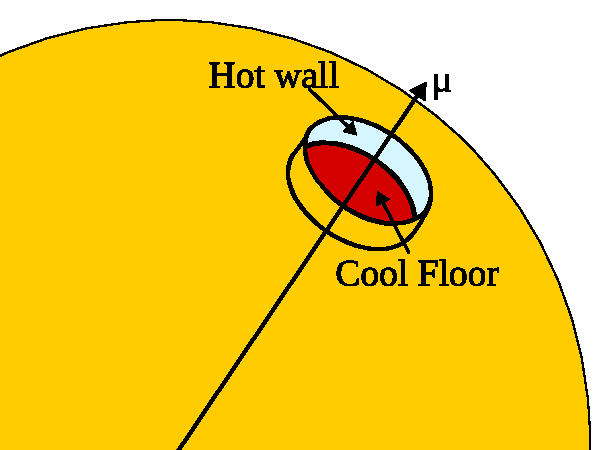
\includegraphics[width=0.5\textwidth]{figures/facula_diagram.pdf}}
    \gridline{\includegraphics[width=0.5\textwidth]{figures/facula_depth.pdf}}
    \script{facula_depth.py}
    \caption{
        ``Hot Wall'' model of faculae. Faculae structure causes their contrast to be dependent on their distance from the center of the disk. {\bf Top}: Depiction of a facula on the limb of a star. The hot wall is exposed to the observer causing the pore to appear bright. At disk center, the cool floor is most visible. {\bf Bottom}: The effects of depression depth and viewing angle on facula brightness. The 3D structure of faculae is most apparent when radius $\sim$ depth. A toy flux model was used to demonstrate the shape of these curves, but in practice their magnitudes depend on stellar spectral models.
        }
    \label{fig:fac_struct}
\end{figure}

\subsection{Flares \label{subsec:flares}}
Flares are an important source of stellar variability on short timescales. \texttt{vspec-vsm}'s flare lightcurve model is based on the \texttt{xoflares} package \citep{barclay2020}, which itself is based on empirically derived lightcurve shapes from \citet{davenport2016}. However, \texttt{xoflares} is designed to fit lightcurves in a single spectral band, so we add additional parameters to extend it to a multiwavelength lightcurve. We completely describe a flare using its temperature, total energy, full width at half maximum (FWHM), and the time of its peak. We model a flare as a hot, optically thin region above the photosphere that produces a blackbody spectrum. In this model, the temperature is constant, and the sharp rise and fall seen in the lightcurve is caused by the region's rapidly changing area. This simplification allows the total flare energy $E$ to be used as a normalization factor:
\begin{equation}
    \int_{-\infty}^{\infty}A\,dt = \frac{E}{\sigma T^4}
\end{equation}
where $A$ is the time-dependent area of the flare region, $T$ is the constant flare temperature, and $\sigma$ is the Stefan-Boltzmann constant. This allows flare lightcurves to be produced with a fixed bolometric luminosity. Because the temperature is fixed, the relevant quantity for modeling the flux of a flare in a given integration is the integrated time-area $\int A\,dt$. These quantities are computed numerically and fed to \vspec{} along with $T$ to produce spectra with the appropriate absolute flux.

Before simulating an observation, \vspec{} asks \texttt{vspec-vsm} to pre-compute a population of flares based on a power-law frequency-energy relationship based on Kepler and TESS lightcurves \citep{gao2022}:
\begin{equation} \label{eq:flare_freq}
    \log{(f/{\rm [day]})} = \beta + \alpha~\log{(E/{\rm [erg]})}
\end{equation}
where $f$ is the frequency of flares with energies $\ge E$. We compute the number of expected flares over a time duration and determine the number to create $N$ by a random Poisson draw. We then generate $N$ flares with energies determined by the quantile function:
\begin{equation}
    E = E_{\text{min}} (1-X)^{1/\alpha}
\end{equation}
where $E_{\text{min}}$ is the minimum considered flare energy and $X$ is a random number on the interval $[0,1)$. We set the default values $\alpha=-0.829$, $\beta=26.87$ from \citet{gao2022}, but these can be adjusted by the user. Figure \ref{fig:flare_freq} shows our simulation results compared to their power-law values.

\begin{figure}
    \centering
    \includegraphics[width=0.5\textwidth]{figures/flare_freq.pdf}
    \caption{
        {\bf Top}: Generated flare frequencies compared to those expected from \citet{gao2022}, generated using a 10,000 day simulation. The $y$-axis shows the frequency of flares with energies greater than or equal to the value of the $x$-axis. Error bars based on the square root of the number of observed flares as this is a Poisson process. {\bf Bottom}: Lightcurve of a star flaring with the same power-law slope as the top panel, but the intercept ($\beta$) has been increased by 0.3 for visual effect. The mean flare temperature is $9000$ K and the mean FWHM is $3$ hours.
        }
    \script{flare_freq.py}
    \label{fig:flare_freq}
\end{figure}

\subsection{Granulation}
Granulation is a source of stellar variability that arises from convection near the surface of the star. The result is a stellar surface that is not constant in temperature and that changes on very short timescales. Hydrodynamic simulations of stellar atmospheres \citep[e.g.][]{magic2014} describe hot granules of rising gas surrounded by cooler, sinking regions with a temperature a few percent lower than the nominal value. 

We model granulation as a global process, and its effects are computed after the effects of spots and faculae. Of the remaining ``quiet'' photosphere (i.e. the regions not covered in spots of faculae), a fraction is computed to be part of the cool
inter-granule surface; the surface coverage of the cool region at any given time is computed by a Gaussian process (GP) using the {\sc tinygp} package \citep{foreman-mackey2024} following the methodology of \citet{gordon2020}. The GP uses a custom kernel function based on a power spectrum \citep{anderson1990,kallinger2014} to produce random changes in the granulation coverage.

\begin{figure}
    \centering
    \includegraphics[width=0.5\textwidth]{figures/granulation_lightcurve.pdf}
    \caption{
        Effect of granulation on the lightcurve of a star. The parameters chosen in this simulation mean that, on average, 10\% of the stellar surface is covered by the cool, inter-granule region with a temperature 300K lower than the surrounding photosphere, and that this coverage varies by about 1\% on a timescale of 6 hours.
        }
    \script{granule_lc.py}
    \label{fig:gran_lc}
\end{figure}

\subsection{Transits \& Limb Darkening}

\begin{figure*}
    \centering
    \includegraphics[width=\textwidth]{figures/ld_transit.pdf}
    \caption{
        {\bf Right}: Transit lightcurves at 1 ${\rm \mu m}$ for a Lambertian (i.e. no limb darkening) star and one with significant limb darkening \citep[$u_1=0.5,\,u_2=0.15$,][]{espinoza2015}. In each case a 1 $R_e$ planet transits a 0.12 $R_\odot$ ($T_{\rm eff} = 3000$ K) star with an observation cadence of 1 minute. Scattered points show the observation with simulated noise, considering a single wavelength channel from JWST/NIRSpec G395H binned to a resolving power of 270 and a target distance of 5 pc.
        {\bf Left}: Stellar surface maps including translucent masks to show limb darkening and transit. The Lambertian star (top) does not exhibit any limb darkening, and its disk has constant surface brightness. However, the limb-darkened star (bottom) is much brighter at disk-center than it is near the limb. The dark circle on the leftmost limb of each star is the region occulted by the planet when it is $0.7^\circ$ from mid-transit.
    }
    \script{ld_transit.py}
    \label{fig:ld_transit}
\end{figure*}

In the case of a transiting geometry, \texttt{vspec-vsm} is responsible for computing the properties of the portion of the stellar disk that is occulted. It does this by first projecting both the transiting planet and the visible part of the surface orthographically as they would be viewed by a distant observer. It then selects all the points that are near enough to the transit to be occulted. The code then iterates through each of those points and computes the fraction of it covered by the occulting circle using a 2D numerical integral. The weight of each point is determined by the geometric projected area as well as a quadratic limb darkening law \citep[see][]{espinoza2015}. This treatment allows the user to specify two parameters $u_1$ and $u_2$ that describe the flux variation as a function of angle from disk-center. A caveat of this method is that there is no dependence on wavelength. A better treatment would vary the temperature of the stellar model as a function of $\mu$; we simply apply a gray scaling factor to the flux. Figure \ref{fig:ld_transit} compares transit lightcurves for two different sets of limb darkening parameters.


\section{Stellar Spectral Grids}
\label{sec:gridpolator}

\begin{figure}
    \centering
    \includegraphics[width=0.5\textwidth]{figures/jax_v_scipy.pdf}
    \caption{
        Speed comparison between the JAX and SciPy implementations of the GridPolator interpolation backend. Both interpolators use the builtin \vspec{} grid, with \teff ranging from 2800 to 3300K, and wavelengths from 5-12 ${\rm \mu m}$ with $R=100$. SciPy is most efficient for a small number of evaluations, with a constant cost per call. For a large number of evaluations, however, the speed gained via JAX's JIT compilation offsets the cost of performing that compilation.
    }
    \script{jax_v_scipy.py}
    \label{fig:jax_v_scipy}
\end{figure}

\vspec{} utilizes a library of pre-computed stellar models for producing its multi-component composite stellar spectrum; detailed stellar spectral models are computationally expensive to generate, so it is more efficient to interpolate over a discretized grid. This interpolation is handled by the VSPEC-related Python package GridPolator, whose main class \texttt{GridSpectra} acts as a wrapper for the SciPy \citep{virtanen2020} or JAX \citep{jamesbradbury2018} \texttt{RegularGridInterpolator} with a specialized API. This setup accomodates spectral grids of arbitrary dimension, and treats the wavelength axis independently of the other parameters so that each wavelength channel is independent. When a \texttt{Gridspectra} instance's \texttt{evaluate()} method is called, it creates a \texttt{RegularGridInterpolator} instance for each wavelength channel, evaluates that interpolator, and then resamples the returned spectrum at the requested wavelength points. In the case that the JAX implementation is used, the portion of \texttt{evaluate()} that does the interpolation is just-in-time (JIT) compiled to dramatically improve performance on subsequent calls. Figure \ref{fig:jax_v_scipy} compares the computational cost of JAX with that of SciPy.

GridPolator grids can be built arbitrarily by the user, but the package comes with a built-in custom grid of \texttt{PHOENIX} stellar models \citep{allard1994,hauschildt1999,husser2013} created specifically for \vspec{}. Each spectrum spans from 0.1 to 20 microns in steps of $5\times10^{-6}$ microns. The stellar atmospheres used to create the spectra have solar metallicity and a $\log{g}$ of 5.0, with effective temperatures ranging from 2300K to 3900K in steps of 100K. Currently this is the only grid currently supported by \vspec{}, with support for additional grids planned in future releases.
% The second grid is hosted by the Space Telescope Science Institute\footnote{\url{https://archive.stsci.edu/hlsps/reference-atlases/cdbs/grid/phoenix/}}. This grid covers a much larger stellar parameter space, with metallicities ranging from $-4$ to $0.5$, \teff from 2000K to 70\,000K, and $\log{g}$ from 0 to 5.5. These models are also produced by the \texttt{PHOENIX} code. Except for the solar metallicity models, the spectra were computed in 2011 by \citet{allard2003, allard2007} and the solar metallicity models were updated by a new version of \texttt{PHOENIX} in 2021 \citep{allard2012}. \TJ{Look up wavelength ranges}
When the grid is initialized, GridPolator looks for the relevant data files on the user's local system. If they are not present, then the files are downloaded and stored in \texttt{\textasciitilde /.gridpolator/grids/}. 

Within this suite of codes, GridPolator has the added responsibility of binning spectra and producing wavelength axes that match those output by PSG. Wavelength sampling is done using constant resolving power $R=\frac{\lambda}{\Delta \lambda}$. The binning algorithm takes a pair of high-resolution flux and wavelength arrays and resamples the flux to a lower-resolution wavelength axis. PSG specifies the central wavelength of each channel, and so this algorithm defines bin edges to be $\lambda_{\rm cen} \pm \frac{\lambda_{\rm cen}}{R}$.

\section{Simplified Climate Model}
\vspec{} allows users to run simulations with any climate model they desire (so long as it can be converted into the \texttt{pypsg.PyGCM} format) and even comes with utilities to work with PSG/GlobES binary files, ExoCAM \citep{wolf2022}, WACCM \citep{marsh2013}, and ExoPlaSim \citep{paradise2022} without any custom code from the user.

However, as a full global circulation model can take days to months to converge, there are many cases where a ``quick and dirty'' 3D climate model may be sufficient. Built into \vspec{} is such a ``faux'' climate model -- one that does not contain any of the circulation physics of the above sophisticated codes, but instead constructs a 3D planetary atmosphere in a fraction of a second from just a few parameters. Such a model can also be advantageous because it is extremely predictable; a feature in the phase curve can easily be traced back to the model parameters that cause it.

The \vspec{} GCM centers around a 2D temperature map of the planet's surface. Based on \citet{cowan2011}, this map
is determined exclusively by the incident flux from the star (parameterized by the host \teff~and radius
and the planet's semimajor axis and Bond albedo) and the unitless thermal redistribution efficiency $\epsilon$.
This efficiency is 0 for a planet that re-radiates instantly and $\gg 1$ for an atmosphere that efficiently redistributes heat to its night side. Figure \ref{fig:thermal_inertia} shows a temperature map example for an Earth-like planet with $\epsilon = 2\pi$. These temperature maps are validated by the energy balance of the planet; \vspec{} computes the incident and emergent flux across the planet and issues a warning if they are not in agreement.

\begin{figure}
    \centering
    \includegraphics[width=0.5\textwidth]{figures/cowan_gcm.pdf}
    \caption{
        Example of a surface temperature map created by the \vspec{} GCM, using values for the solar flux equivalent to Earth, a Bond albedo of 0.3, and $\epsilon = 2\pi$. Notice that the hottest point is offset from the sub-stellar point due to thermal inertia.
    }
    \script{cowan_gcm.py}
    \label{fig:thermal_inertia}
\end{figure}

To compute the surface temperature we first compute the temperature at the equator as a function of longitude. This is done by integrating Equation (10) of \citet{cowan2011}
\begin{equation}
    \frac{d \tilde{T}}{d \Phi} = \frac{1}{\epsilon}(\max{(\cos{\Phi}, 0)} - \tilde{T}^4)
\end{equation}
Where $\tilde{T}$ is the dimensionless temperature defined as $T/T_0$, or the temperature normalized by a local fiducial value. $\Phi$ is the angle from the substellar point, so we numerically integrate it from $-\pi$ to $\pi$ using one of several different schemes depending on the value of $\epsilon$. For $0 < \epsilon < 1$ we adopt a reflecting initial value problem (IVP) scheme, where we set $\tilde{T}=1$ at $\Phi=\pi$, integrate to $-\pi$, then use the last value as the initial value for an integration from $-\pi$ to $\pi$. Note that for extremely small values of $\epsilon$ (e.g. $10^{-6}$), the integration is slow, and will fail if $\epsilon=0$; we recommended a lower limit of $\epsilon=10^{-4}$. When $1\le \epsilon < 10$ we solve the integral using a boundary value problem (BVP) scheme. For each of these two methods we employ the SciPy \citep{virtanen2020} implementation: \texttt{solve\_ivp()}, employing a 5th order Runga-Kutta scheme \citep{dormand1980} and \texttt{solve\_bvp()}, based on an earlier MATLAB implementation \citep{kierzenka2001}, respectively. When $\epsilon \ge 10$ it is more efficient to use the analytic approximation given by Equation (A2) in \citet{cowan2011}. In Figure \ref{fig:cowan_curves} we show results for several different values of $\epsilon$.

\begin{figure}
    \centering
    \includegraphics[width=0.5\textwidth]{figures/cowan_fig1.pdf}
    \caption{
        {\bf Top}: Reproduction of \citet{cowan2011} Figure 1 using the methods described in the text. These curves show the dimensionless temperature at the equator of a planet as a function of angle from substellar point $\Phi$ for thermal inertia $\epsilon$. Note that the $\epsilon=0$ curve in the original figure is replaced with $\epsilon=10^{-4}$ (see explanation in the text), and we do not include additional curves for mid-latitudes as in the original figure. As $\epsilon$ increases, heat is moved from the dayside onto the nightside and the temperature maximum shifts away from the substellar point.
        {\bf Bottom}: Relative surface temperature as a function of latitude $\lambda$ for varying latitudinal mixing parameter $\alpha$. A value of 1 means the equatorial temperature as computed in the upper panel. Without mixing ($\alpha=0$) heat is concentrated at the Equator. However, as $\alpha$ increases, the equator cools and heat is redistributed towards the poles.
    }
    \script{cowan_fig.py}
    \label{fig:cowan_curves}
\end{figure}

\subsection{Extending to 3 Dimensions}

The treatment by \citet{cowan2011} includes no mixing in the latitudinal direction, nor a vertical temperature profile; to allow for variations in pressure and inclination, we augment their treatment with several simple approximations for latitudinal and vertical temperature variations. 

We add a parameter $\alpha$ that is defined by the ratio between the polar temperature and the equatorial temperature at any given longitude. We define $f(\lambda;\alpha)$ to be the temperature as a function of latitude $\lambda$ at an arbitrary longitude; therefore if the surface is in equilibrium, the energy balance requires the outgoing energy flux to be independent of $\alpha$:
\begin{equation}
    \label{eq:e_out}
    E_{\rm out} = \sigma \int_0^{\pi/2} f(\lambda; \alpha)^4 \cos{\lambda}\,d\lambda
\end{equation}
where $E_{\rm out}$ is the outbound energy flux of an infinitesimal sliver of differential longitude. In the case of $\alpha=0$ (i.e. no mixing) we can treat each latitude value independently, so the equilibrium temperature is
\begin{equation}
    f(\lambda; 0) = f(0;0) \cos^{1/4}{\lambda}
\end{equation}
where $f(0;0)$ is the previously computed temperature at the equator (see Figure \ref{fig:cowan_curves}). Plugging this in to Equation (\ref{eq:e_out}), we see
\begin{equation}
    \label{eq:nomix}
    \begin{array}{cl}
        E_{\rm out} & = \sigma \int_0^{\pi/2} (f(0;0) \cos^{1/4}{\lambda})^4\cos{\lambda}\,d\lambda \\
        & = \sigma f^4(0;0) \int_0^{\pi/2} \cos^{2}{\lambda}\,d\lambda \\
        & = \frac{\pi}{4}\sigma f^4(0;0)
    \end{array}
\end{equation}

If instead we let $f(\lambda;1)$ be a constant function where the equator and pole have equal temperatures, then
\begin{equation}
    \label{eq:allmix}
    \begin{array}{cl}
        E_{\rm out} & = \sigma \int_0^{\pi/2} f(\lambda;1)^4 \cos{\lambda}\,d\lambda \\
        & = \sigma f^4(0;1) \int_0^{\pi/2} \cos{\lambda}\,d\lambda \\
        & = \sigma f^4(0;1)
    \end{array}
\end{equation}

We calculate $f(0,1)$ by setting Equations (\ref{eq:nomix} \& \ref{eq:allmix}) equal to find
\begin{equation}
    f(0;1) = \left(\frac{\pi}{4}\right)^{1/4} f(0;0) \approx 0.94 \,f(0;0)
\end{equation}

We can now write a general parameterization for the temperature as a function of latitude
\begin{equation}
    \label{eq:temp_gen}
    f(\lambda;\alpha) = f(0;0)\,\left(\alpha \frac{\pi}{4} + (1-\alpha) \cos{\lambda}\right)^{1/4}
\end{equation}

%\subsection{Pressure and Temperature}
Combining Equation (\ref{eq:temp_gen}) with the numerically-computed equatorial temperatures yields a 2D temperature map that covers the surface of the planet. We construct a 3D atmosphere on top of this surface assuming the atmosphere is adiabatic with index $\gamma$. The user supplies both the adiabatic index and the surface pressure $P_{\rm surf}$. The temperature at some altitude $z$ is given by
\begin{equation}
    T_z = T_{\rm surf}\,\left( \frac{P_z}{P_{\rm surf}} \right)^{1-\frac{1}{\gamma}}
\end{equation}

Finally, we populate our atmosphere with molecules. The user specifies the species and abundance and atmosphere is filled accordingly with a constant molecular suite.

\section{Examples \label{sec:examples}}

\subsection{Transit of a spotted star}

In this section we will simulate the transit of a bare rock across a spotted star to demonstrate how an inhomogeneous
stellar surface can lead to a false atmospheric signal -- a phenomenon known as the ``transit light source effect'' \citep{rackham2018}.
During transit, the planetary atmosphere is illuminated by the portion of the star directly behind the planet. The depth of the transit
should be measured with respect for the spectrum of this region of the stellar surface. However, the disk-integrated stellar spectrum is often used instead.
In the case that the stellar surface is not homogeneous, the transit signal is contaminated by the star.
\citet{moran2023} first observed this effect using JWST from super-Earth GJ 486b.

Whenever possible, we draw parameter values from \citet{moran2023} and the NExScI Archive\footnote{\url{https://exoplanetarchive.ipac.caltech.edu/overview/GJ1214b}}.
We use the JWST NIRSpec/G395H instrument setup but set $R=200$ to account for the resolution of the reduction.
Additionally we observe for 3.53 hours with an 8 minute cadence. Mid-transit is reached exactly halfway through the observation.

We will do three \vspec{} simulations:
\begin{enumerate}
    \item Bare rock, no spots.
    \item 1 bar \ce{H2O} atmosphere, no spots.
    \item Bare rock, 2.5\% coverage by 2700 K spots
\end{enumerate}

We expect in case 1 to observe a flat spectrum, and in case 2 to observe additional
absorption from the \ce{H2O} atmosphere. Note also that we disabled \ce{H2O}-\ce{H2O} collision-induced absorption (CIA) for
these simulations because the effect was not considered in the original analysis of GJ 486b.

\begin{figure}
    \centering
    \includegraphics[width=0.5\textwidth]{figures/moran23.pdf}
    \caption{
        The results from our spotted transit experiment. We find that the addition of
        spots to a star's surface can give an otherwise flat transit spectrum features that appear to be molecular bands.
        This is in agreement with the results of \citet{moran2023}.
        }
    \script{moran23.py}
    \label{fig:moran_transit}
\end{figure}

We find that, as expected, the addition of spots changes the transit depth in a way that depends on wavelength -- mimicking
light lost to absorbers in a planetary atmosphere. Figure \ref{fig:moran_transit} shows us that, in this case, we observe false absorption;
this is due to an increase in the spotted fraction of the surface relative to the quiet photosphere. However, if a spot was blocked by
the planet we might see similar features inverted to mimic emission.

\subsection{Phase Curve}
Analysis of JWST MIRI-LRS phase curves of GJ 1214b by \citet{kempton2023} did not consider stellar
contamination because of the slow rotation rate of the host star \citep[approximately 1/80$^{\text{th}}$ the orbital frequency,][]{cloutier2021}.
In this example we use \vspec{} to demonstrate that this is a reasonable assumption.

We initialize \vspec{} to run a 41.0 hour observation with a cadence of 15 minutes. We use stellar and planetary parameters
from the NExScI Exoplanet Archive\footnote{\url{https://exoplanetarchive.ipac.caltech.edu/overview/GJ1214b}}.
The GCM used has a thermal inertia of $\epsilon = 6$ and a 1 bar \ce{CO2} atmosphere.

We initialized two stellar models: one with nothing more than a 3250 K surface, and another with 20\% coverage by 2700 K spots.

After running the \vspec{} simulations, we bin into 0.5 $\mu m$ wavelength channels and normalize each channel to the two eclipses.
We assume the star behaves linearly between eclipse measurements and attribute any deviation to the planet.

\begin{figure}
    \centering
    \includegraphics[width=0.5\textwidth]{figures/kempton23.pdf}
    \caption{
        MIRI phase curves for GJ 1214b binned by wavelength. Compare to \citet{kempton2023} Extended Data Figure 1.
        While the addition of stellar variability does have a visible effect on the lightcurve, it is much smaller than the thermal emission by the exoplanet.
        }
    \script{kempton23.py}
    \label{fig:gj1214b}
\end{figure}

We show in Figure \ref{fig:gj1214b} that the stellar properties assumed in this example do not generate enough contamination to
significantly change the observed phase curve of GJ 1214b. At it's worst (i.e. near transit) the observed spectrum varies by 50 ppm due to stellar
contamination -- compared to the 700 ppm relative flux of the planet at $8.5 {\mu m}$. Similar studies could be done to assess the potential for
stellar contamination in other exoplanetary systems in order to judge fitness as a target.

% \subsection{MIRECLE Phase Curve}
% In this example we will look at the best-case target for the Mid-IR Exoplanet CLimate Explorer \citep[MIRECLE,][]{mandell2022}
% mission concept: Proxima Centauri b with no stellar variability. We will instead examine the expected noise produced by this observation
% and assess the detectability of the planet in a single orbit. \vspec{} uses the noise models built into PSG, allowing native support for
% noise due to the instrument, source, and astrophysical background.

% We use \vspec{}'s built-in MIRECLE instrument template, which includes a 2 m aperture and observes from 1-18 $\mu m$ with $R=50$.
% We draw stellar and bulk planetary parameters from the NExScI Exoplanet Archive\footnote{\url{https://exoplanetarchive.ipac.caltech.edu/overview/proxima\%20cen}}
% and assume $i=85^\circ$ and Earth density. The GCM we use has a Bond albedo of 0.3, $\epsilon=1.5$, $P_{\rm surf} = 1 \text{bar}$ and a 100 ppm \ce{CO2} atmosphere with a \ce{N2} background.
% We ran the simulation for one orbit with an 24 hour cadence. Because this is a best-case scenario, we assumed perfect knowledge of the stellar spectrum.
% We are left with the planetary spectrum and photon noise from the star.

% \begin{figure}
%     \centering
%     \includegraphics[width=0.5\textwidth]{figures/mirecle.pdf}
%     \caption{
%         Simulated spectra of Proxima Centauri b observed by MIRECLE. Noise and error bars based on 24 hour integrations with a 2 m aperture MIRECLE
%         space telescope.
%         }
%     \script{mirecle.py}
%     \label{fig:mirecle}
% \end{figure}

\section{Conclusion \label{sec:conclusion}}
\TJ{Talk about what we can do next.}

\bibliography{syw,VSPEC}

\end{document}
